\subsection{The fundamental domain and the tessellation of the halfplane}

We have seen in Remark~\ref{rem_NatureMoebius} that considering M�bius transformations as meromorphic functions $\EC \to \EC$ very naturally induces a group action of $\PGL{\C}$ on $\EC$. Clearly this group action is also given for any subgroup of $\PGL{\C}$ and in particular for the modular group. 

For the following it will be convenient to write modular transformations in matrix form and the elements $z \in \EC$ as quotients $z = u/v$ for suitable $u,v \in \C$, not both zero. A formal quotient $u/0$ will be identified with $\infty$. In this notation, for a modular transformation $A = \smallmat{a}{b}{c}{d} \in \PSL{\Z}$ and $u/v \in \EC$ the mentioned group action is given by
\begin{equation}
\label{eqn_ModGrpAction}
A \ \frac{u}{v} := \frac{a u + b v}{c u + d v}
\end{equation}
We call two points $z, w \in \EC$ \emph{equivalent}, if and only if there is a modular transformation $A \in \PSL{\Z}$ with $A z = w$ and we write  $z \sim w$. The equivalence class (\emph{orbit}) of a point $u/v \in \EC$ is given by 
\begin{equation*}
\left[\frac{u}{v}\right]_\sim = 
\setdefsz{\bigg}{\frac{a u + b v}{c u + d v} \in \EC}{\mat{a}{b}{c}{d} \in \PSL{\Z}} \in \EC / \sim.
\end{equation*}

We now wish to find a system of representatives for $\EC/\sim$, in other words, we want to define exactly one representative $u_0/v_0$ for each orbit $[u/v]_\sim$. One approach for this could be to fix $u,v \in \C$, not both zero, then to choose from the set
\begin{equation}
\label{eqn_FunDomOuv}
O_{u,v} := \setdefsz{\bigg}{\cvec{a u + b v}{c u + d v} \in \C^2}{\mat{a}{b}{c}{d} \in \SL{\Z}}
\end{equation}
one vector $(u_0, v_0)$ with minimal $\eucnorm{\cdot}$-norm and to declare $u_0/v_0$ as the representative for $[u/v]_\sim$. The problem with this is that such a choice may not always be possible, because $L_{u,v}$ may in general contain vectors of arbitrary small $\eucnorm{\cdot}$-norm. 

However, if $u \conj{v} \notin \R$, then $u$ and $v$ span a non-degenerate parallelogram $P_{u,v} := \setdef{t u + s v}{t,s \in [0,1)} \subseteq \C$. Translation of $P_{u,v}$ by integer multiples of $u$ and $v$ covers every point in $\C$ exactly once. The set
\begin{equation*}
L_{u,v} := \setdef{a u + b v \in \C}{a,b \in \Z}
\end{equation*}
consists precisely of the vertices of all of these translated parallelograms.\footnote{$L_{u,v}$ forms a lattice in $\C$.} If we denote by $D_r := \setdef{z \in \C}{\abs{z} \le r}$ a disk of radius $r$ centered at the origin, then for every $r > 0$ the set $D_r \cap L_{u,v}$ is obviously finite. 

Now, still for the case $u \conj{v} \notin \R$, we show that the set $O_{u,v} \subseteq (L_{u,v})^2$ must contain an element of minimal $\eucnorm{.}$-norm: Define $S_r := \setdef{x \in \C^2}{\eucnorm{x} \le r}$ and let $r > 0$ be sufficiently large such that $S_r \cap O_{u,v}$ is nonempty. Because 
\begin{equation*}
S_r \cap O_{u,v} \subseteq (D_r \cap L_{u,v})^2,
\end{equation*}
we see that $S_r \cap O_{u,v}$ is finite and $\min \eucnorm{S_r \cap O_{u,v}} = \min \eucnorm{O_{u,v}}$ exists. Since $(0,0) \notin O_{u,v}$ this minimum is not zero.

This encourages us to go on (we will come back to the case $u \conj{v} \in \R$ later) and turn to the question, how we can effectively determine an element of $O_{u,v}$ with minimal $\eucnorm{\cdot}$-norm. The task is the following: Given two complex numbers $u,v \in \C$ with $u \conj{v} \notin \R$, determine a matrix $A \in \SL{\Z}$ such that $\eucnorm{A ({}^u_v)}$ is minimal. In Theorem~\ref{thm_ModGrpTUGen} we have seen that $\PSL{\Z}$ is generated by ${}_\pm T$ and ${}_\pm U$.\footnote{Here, for clarity, we again use the notation ${}_\pm M := M_\sim = \{\pm M\} \in \PSL{\Z}$ to distinguish from the matrix $M \in \SL{\Z}$.} As a consequence,  $\SL{\Z}$ is generated by the matrices $T = \smallmat{0}{-1}{1}{\phantom{-}0}$, $U = \smallmat{1}{1}{0}{1}$ and $N = -\smallmat{1}{0}{0}{1}$. The idea is now to successively multiply $({}^u_v)$ with appropriate powers of $T$ and $U$ to obtain vectors of smaller and smaller $\eucnorm{\cdot}$-norm (multiplying with $N$ would not help us in this regard). We do this by first determining $q_0 \in \Z$, such that $\eucnorm{U^{-q_0} ({}^u_v)}$ is minimal -- the following trivial lemma helps us with this:
\begin{lemma}
\index{nint@nint (Nearest integer function)}
Let $u,v \in \C$ with $v \ne 0$ and $q \in \Z$. The statements
\begin{enumerate}[\qquad(i)]
\item \label{itm_uvMini}
$q$ minimizes $\eucnorm{U^{-q}\cvec{u}{v}} = \eucnorm{\cvec{u - q v}{v}}$,
\item \label{itm_uvMinii} $q$ minimizes $\abs{u - q v}$,
\item \label{itm_uvMiniii} $q$ minimizes $\abs{\frac{u}{v} - q}$,
\item \label{itm_uvMiniv} $q = \nint{\Re{\frac{u}{v}}}$,
\end{enumerate}
satisfy $(\ref{itm_uvMini}) \Leftrightarrow (\ref{itm_uvMinii}) \Leftrightarrow (\ref{itm_uvMiniii})$ and $(\ref{itm_uvMiniv}) \Rightarrow (\ref{itm_uvMiniii})$.
In the last statement, $\operatorname{nint}$ stands for the \emph{nearest integer function}, \ie for rounding to the nearest integer.
\end{lemma}
After fixing such a $q_0 \in \Z$, we multiply with $T$ and repeat the process for finding $q_1 \in \Z$ minimizing $\eucnorm{U^{q_1} T U^{q_0} ({}^u_v)}$ and so on. The process ends, when $q_n = 0$ for some $n>0$.

\begin{theorem}
\label{thm_FunDomUVAlg}
Let $u,v \in \C$ with $u \conj{v} \notin \R$. A matrix $A \in \SL{\Z}$ minimizing $\eucnorm{A ({}^u_v)}$ can be found by performing the following steps:
\begin{enumerate}
\item Set $(r_{-1},r_0) := (u,v)$ and $j := 0$.
\item \label{itm_FunDomUVAlgLoop}
Determine $q_j := \nint{\Re{\frac{r_{j-1}}{r_j}}}$.
\item If $j > 0$ and $q_j = 0$ go to step \ref{itm_FunDomUVAlgDone}. Otherwise, set $r_{j+1} := r_{j-1} - q_j r_j$, increment $j$ by one and continue with step \ref{itm_FunDomUVAlgLoop}.
\item \label{itm_FunDomUVAlgDone} Set $n := j-1$. For $i \in \{0,1,\dots,n\}$, set $e_i := (-1)^i q_i$. The desired matrix is
\begin{equation*}
A = U^{e_0} TU^{e_1} \cdots TU^{e_n}.
\end{equation*}
\end{enumerate}
\end{theorem}
\begin{proof}
The algorithm gives rise to a sequence of equations
\begin{eqnarray*}
      u &=& q_0 \cdot v\phantom{_0} + r_1 \\
      v &=& q_1 \cdot r_1 + r_2 \\
    r_1 &=& q_2 \cdot r_2 + r_3 \\
        &\vdots& 
\end{eqnarray*}
The condition $u \conj{v} \notin \R$ implies that $u$ and $v$ are both nonzero and $\frac{u}{v} \notin \R$, \ie $u$ and $v$ are linear independent over $\R$. Since all $r_j$, $j \ge 1$ are nontrivial linear combiniations of $u = r_{-1}$ and $v = r_0$ with integer coefficients, they are all nonzero.  For this reason $r_j \ne 0$ for all $j \ge -1$. Also the integers $q_j$ with the possible exception of $q_0$ and of course $q_n$, if the algorithm terminates and $n$ is defined, are nonzero. From $r_{j+1} = r_{j-1} - q_j r_j$ we see
\begin{equation*}
\abs{r_{j+1}} \le \abs{r_{j-1}} + \abs{q_j} \abs{r_j}
\end{equation*}
\end{proof}

\begin{figure}
\centering
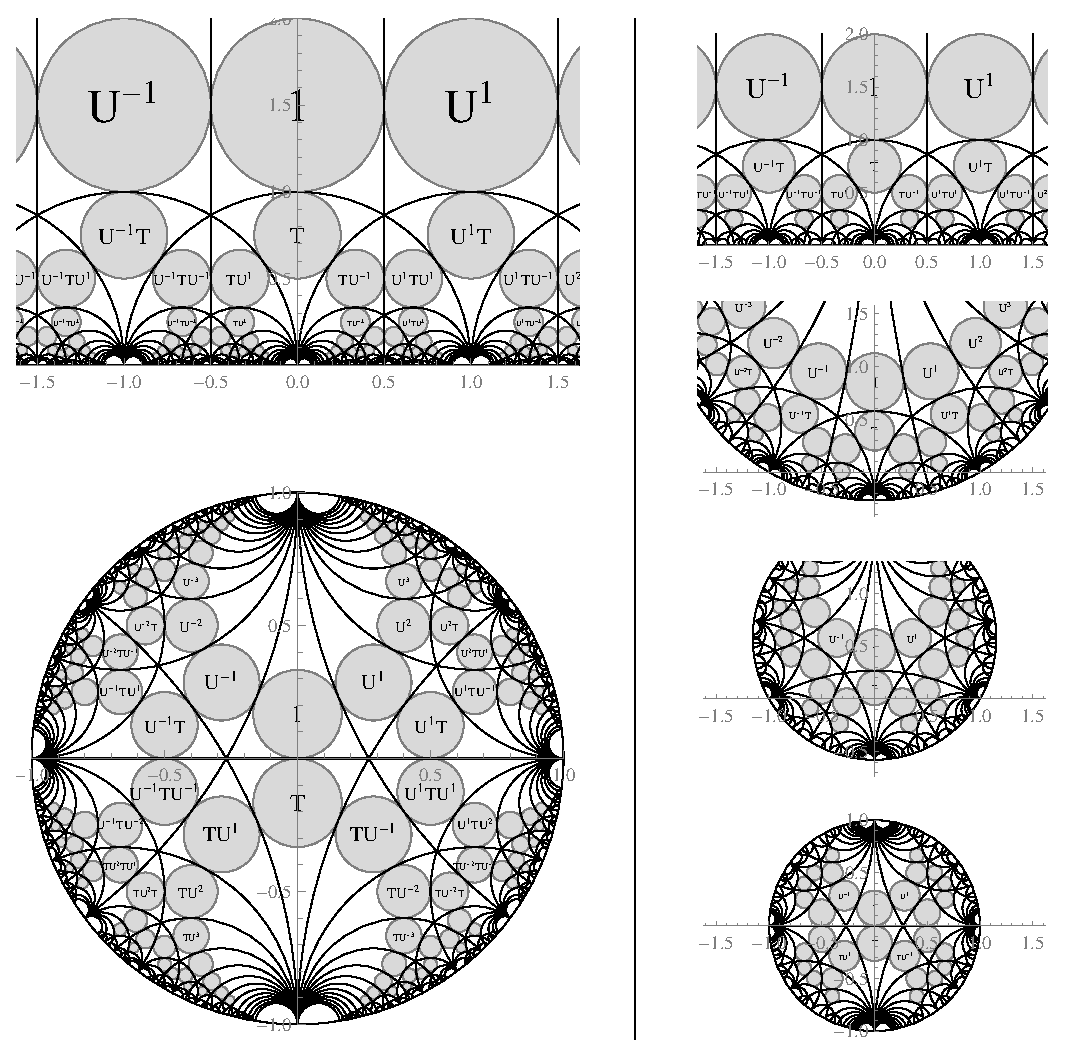
\includegraphics[width=\textwidth]{figures/modular-tiling-1}
\caption{The tessellation of the upper halfplane.}
\label{fig_ModularTiling}
\end{figure}

\begin{figure}
\centering
\includegraphics[width=0.8\textwidth]{figures/modular-tiling-exp-fan}
\caption{The tessellation under the transformation $z \mapsto \exp(2 \pi \ii z)$.}
\label{fig_ModularTilingExpFan}
\end{figure}

\begin{figure}
\centering
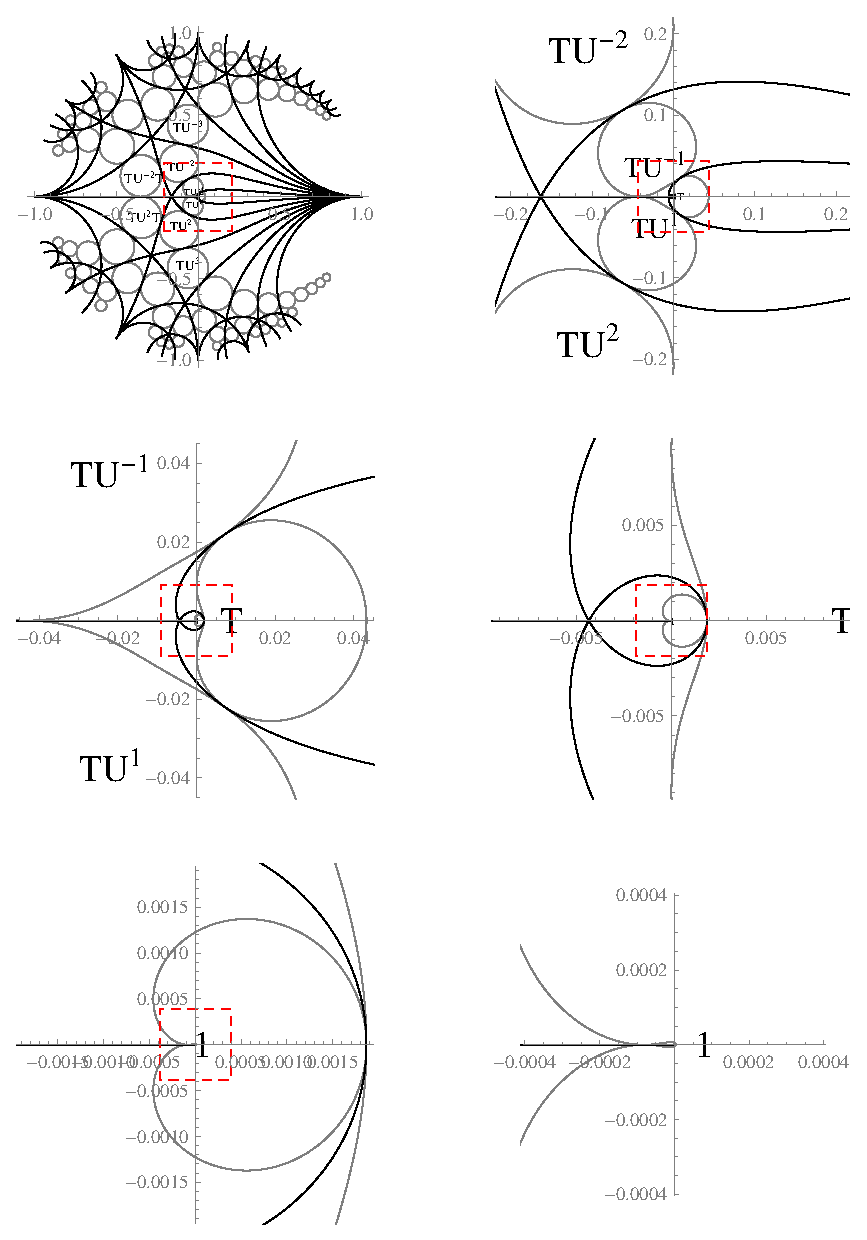
\includegraphics[width=0.8\textwidth]{figures/modular-tiling-exp-zoom}
\caption{The image of the modular tiling under the map $z \mapsto \exp(2 \pi \ii z)$ in the neighborhood of $\infty$.}
\label{fig_ModularTilingExpZoom}
\end{figure}
